
\pdfminorversion=4 % for acroread
%\documentclass[aspectratio=169,t,xcolor={usenames,dvipsnames}]{beamer}
\documentclass[aspectratio=169,t,handout,xcolor={usenames,dvipsnames}]{beamer}
\usepackage{../beamerstyle}
\usepackage{dsfont}
\usepackage{bm}
\usepackage[english]{babel}
\usepackage[utf8]{inputenc}
\usepackage{graphicx}
\usepackage{algorithm}
\usepackage[ruled,vlined,algo2e,linesnumbered]{algorithm2e}
%\usepackage[boxed,vlined]{algorithm2e}
\usepackage{hyperref}
\usepackage{booktabs}
\usepackage{mathtools}

\usepackage{amsmath,amssymb}
\usepackage{listings}
\lstset{frame=lines,framesep=3pt,numbers=left,numberblanklines=false,basicstyle=\ttfamily\small}

\usepackage{subfig}
\usepackage{multicol}
%\usepackage{appendixnumberbeamer}
%
\usepackage{tcolorbox}

\usepackage{pgfplots}
\usepackage{tikz}
\usetikzlibrary{trees} 
\usetikzlibrary{shapes.geometric}
\usetikzlibrary{positioning,shapes,shadows,arrows,calc,mindmap}
\usetikzlibrary{positioning,fadings,through}
\usetikzlibrary{decorations.pathreplacing}
\usetikzlibrary{intersections}
\usetikzlibrary{positioning,fit,calc,shadows,backgrounds}
\pgfdeclarelayer{background}
\pgfdeclarelayer{foreground}
\pgfsetlayers{background,main,foreground}
\tikzstyle{activity}=[rectangle, draw=black, rounded corners, text centered, text width=8em]
\tikzstyle{data}=[rectangle, draw=black, text centered, text width=8em]
\tikzstyle{myarrow}=[->, thick, draw=black]

% Define the layers to draw the diagram
\pgfdeclarelayer{background}
\pgfdeclarelayer{foreground}
\pgfsetlayers{background,main,foreground}

%\usepackage{listings}
%\lstset{numbers=left,
%  showstringspaces=false,
%  frame={tb},
%  captionpos=b,
%  lineskip=0pt,
%  basicstyle=\ttfamily,
%%  extendedchars=true,
%  stepnumber=1,
%  numberstyle=\small,
%  xleftmargin=1em,
%  breaklines
%}

 
\definecolor{blue}{RGB}{0, 74, 153}

\usetheme{Boadilla}
%\useinnertheme{rectangles}
\usecolortheme{whale}
\setbeamercolor{alerted text}{fg=blue}
\useoutertheme{infolines}
\setbeamertemplate{navigation symbols}{\vspace{-5pt}} % to lower the logo
\setbeamercolor{date in head/foot}{bg=white} % blue
\setbeamercolor{date in head/foot}{fg=white}
\setbeamercolor{author  in head/foot}{bg=white} %blue
\setbeamercolor{title in head/foot}{bg=white} % blue
\setbeamercolor{title}{fg=white, bg=blue}
\setbeamercolor{block title}{fg=white,bg=blue}
\setbeamercolor{block body}{bg=blue!10}
\setbeamercolor{frametitle}{fg=white, bg=blue}
\setbeamercovered{invisible}

\makeatletter
\setbeamertemplate{footline}
{
  \leavevmode%
  \hbox{%
  \begin{beamercolorbox}[wd=.333333\paperwidth,ht=2.25ex,dp=1ex,center]{author in head/foot}%
%    \usebeamerfont{author in head/foot}\insertshortauthor
  \end{beamercolorbox}%
  \begin{beamercolorbox}[wd=.333333\paperwidth,ht=2.25ex,dp=1ex,center]{title in head/foot}%
    \usebeamerfont{title in head/foot}\insertshorttitle
  \end{beamercolorbox}%
  \begin{beamercolorbox}[wd=.333333\paperwidth,ht=2.25ex,dp=1ex,right]{date in head/foot}%
    \usebeamerfont{date in head/foot}\insertshortdate{}\hspace*{2em}
%    \insertframenumber\hspace*{2ex} 
  \end{beamercolorbox}}%
  \vskip0pt%
}
\makeatother

%\pgfdeclareimage[height=1.2cm]{automl}{images/logos/automl.png}
%\pgfdeclareimage[height=1.2cm]{freiburg}{images/logos/freiburg}

%\logo{\pgfuseimage{freiburg}}

\renewcommand{\comment}[1]{
	\noindent
	%\vspace{0.25cm}
	{\color{red}{\textbf{TODO:} #1}}
	%\vspace{0.25cm}
}
\newcommand{\notefh}[1]{\textcolor{red}{\textbf{FH:} #1}}
\renewcommand{\comment}[1]{}
\newcommand{\hide}[1]{}
\newcommand{\cemph}[2]{\emph{\textcolor{#1}{#2}}}

\newcommand{\lit}[1]{{\footnotesize\color{black!60}[#1]}}

\newcommand{\litw}[1]{{\footnotesize\color{blue!20}[#1]}}


\newcommand{\myframe}[2]{\begin{frame}[c]{#1}#2\end{frame}}
\newcommand{\myframetop}[2]{\begin{frame}{#1}#2\end{frame}}
\newcommand{\myit}[1]{\begin{itemize}#1\end{itemize}}
\newcommand{\myblock}[2]{\begin{block}{#1}#2\end{block}}


\newcommand{\votepurple}[1]{\textcolor{Purple}{$\bigstar$}}
\newcommand{\voteyellow}[1]{\textcolor{Goldenrod}{$\bigstar$}}
\newcommand{\voteblue}[1]{\textcolor{RoyalBlue}{$\bigstar$}}
\newcommand{\votepink}[1]{\textcolor{Pink}{$\bigstar$}}

\newcommand{\diff}{\mathop{}\!\mathrm{d}}
\newcommand{\refstyle}[1]{{\small{\textcolor{gray}{#1}}}}
\newcommand{\hands}[0]{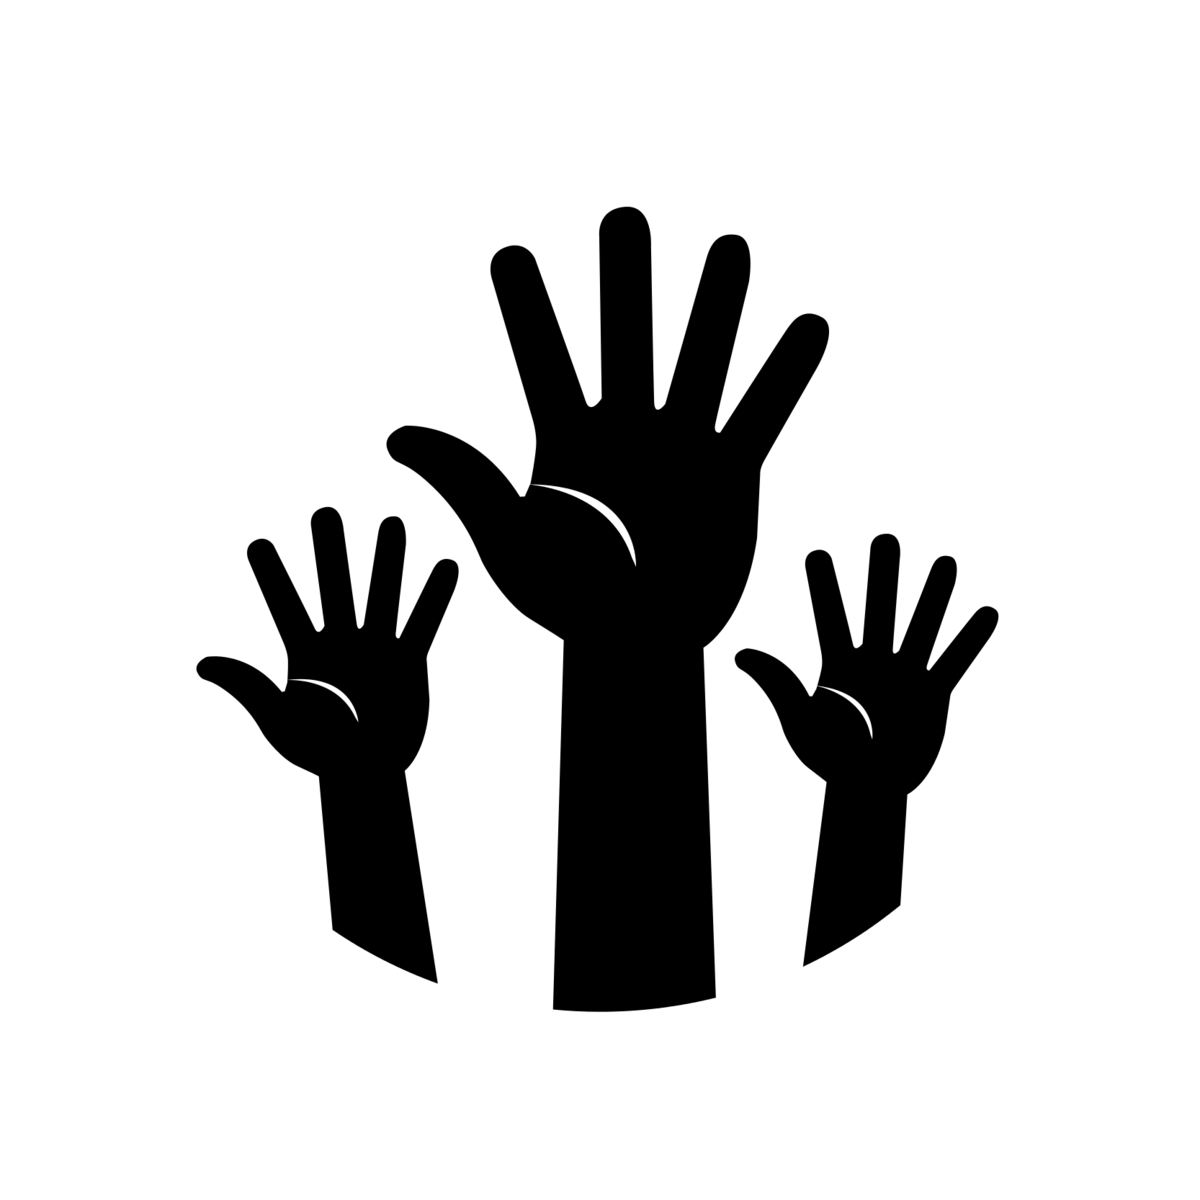
\includegraphics[height=1.5em]{images/hands}}
\newcommand{\transpose}[0]{{\textrm{\tiny{\sf{T}}}}}
\newcommand{\norm}{{\mathcal{N}}}
\newcommand{\cutoff}[0]{\kappa}
\newcommand{\instD}[0]{\dataset}
\newcommand{\insts}[0]{\mathcal{I}}
\newcommand{\inst}[0]{i}
\newcommand{\instI}[1]{i^{(#1)}}

% Iteration specific instance of variable/function/anything
% Introduced in the BO section, but moved up here to make it available within other macros
\newcommand{\iter}[2][\bocount]{{#2}^{(#1)}}

%--------HPO parameter macros-----------

% Parameter Configuration Space
\newcommand{\pcs}[0]{\pmb{\Lambda}}

% ???
\newcommand{\bx}[0]{\conf}

% Parameter Configuration
\newcommand{\conf}[0]{\pmb{\lambda}}

% Final Configuration
\newcommand{\finconf}[0]{\pmb{\hat{\lambda}}}

% Configuration corresponding to a given iteration -- better use \iter!
\newcommand{\confI}[1]{{\conf}^{(#1)}}

% Default Configuration
\newcommand{\defconf}[0]{{\conf}_{\text{def}}}

% Incumbent Configuration
\newcommand{\incumbent}[1][\bocount]{\iter[#1]{\finconf}}

% Optimal Configuration
\newcommand{\optconf}[0]{{\conf}^*}

% Configuration Space
\newcommand{\confs}[0]{\pcs}

%----------------------------------------

%\newcommand{\vlambda}[0]{\bm{\lambda}}
%\newcommand{\vLambda}[0]{\bm{\Lambda}}
\newcommand{\dataset}[0]{\mathcal{D}}
\newcommand{\datasets}[0]{\mathbf{D}}
\newcommand{\loss}[0]{L}
\newcommand{\risk}{\mathcal{R}}
\newcommand{\riske}{\mathcal{R}_{\text{emp}}}
\newcommand{\cost}[0]{c}
\newcommand{\costI}[1]{c^{(#1)}}

% Gaussian Process
\newcommand{\gp}{\mathcal{G}}
% Family of Objective Functions
\newcommand{\objF}{F}

%---------------BO Macros------------------

% BO loop counter
\newcommand{\bocount}{t}
% BO loop counter max, the counter runs from 1 to this value
\newcommand{\bobudget}{T}
% BO loop observation
\newcommand{\obs}[1][\conf]{\cost({#1})}
% BO loop observation space
\newcommand{\obsspace}{\mathcal{Y}}
% BO loop next observation
\newcommand{\bonextobs}{\obs[\iter{\conf}]}
% Acquisition Function, no args
\newcommand{\acq}{u}
% Standard Normal PDF
\newcommand{\pdf}{\phi}
% Standard Normal CDF
\newcommand{\cdf}{\Phi}
% Mean
\newcommand{\mean}{\mu}
% Standard Deviation
\newcommand{\stddev}{\sigma}
% Variance
\newcommand{\variance}{\sigma^2}
% Noise
\newcommand{\noise}{\nu}
% BO loop next selected sample
\newcommand{\bonextsample}{\confI{\bocount}}

% Single hyperparameter
\newcommand{\hyperparam}{\lambda}

% Single hyperparameter within a hyperparameter configuration
\newcommand{\hyperparami}[1][i]{{\hyperparam}_#1}

% Full definition of final configuration
\newcommand{\finconffull}{\incumbent[\bobudget]}

% Dataset
\newcommand{\datasetHPO}{{\dataset}_{HPO}}

% Dataset definition
\newcommand{\datasetHPOdef}{{\langle \bonextsample,\,\bonextobs \rangle}_{\bocount=1}^{\bobudget}}

% Double Display Fraction, forces large displays for everything in numerator and denominator
\newcommand\ddfrac[2]{\frac{\displaystyle #1}{\displaystyle #2}}

% Conditional Probability "Given That" Relation, source:https://tex.stackexchange.com/a/141685/205886
\newcommand\given[1][]{\:#1\vert\:}

% Expectation as a math operator
\DeclareMathOperator*{\E}{\mathbb{E}}

% Citation 
\newcommand{\source}[1]{
    \begin{flushright}
    	Source: \lit{#1}
    \end{flushright}
}
%-------------------------------------------

%Real numbers set
\newcommand{\realnum}{\mathbb{R}}
%Configuration space - do not use
%\newcommand{\configspace}{\Theta}
%Instances - do not use
%\newcommand{\instances}{\mathcal{I}}
%Expected value
\newcommand{\expectation}{\mathbb{E}}
%Kernel
\newcommand{\kernel}{\kappa}
%Constraint function
\newcommand{\constraintf}{c}
%Normal distribution
\newcommand{\normaldist}{\mathcal{N}}

% \renewcommand{\vec}[1]{\mathbf{#1}}
\newcommand{\hist}[0]{\dataset_{\text{Hist}}}
\newcommand{\param}[0]{p}
\newcommand{\algo}[0]{\mathcal{A}}
\newcommand{\algos}[0]{\mathbf{A}}
%\newcommand{\nn}[0]{N}
\newcommand{\feats}[0]{\mathcal{X}_{\text{meta}}}
\newcommand{\feat}[0]{\x_{\text{meta}}}
%\newcommand{\cluster}[0]{\vec{h}}
%\newcommand{\clusters}[0]{\vec{H}}
\newcommand{\perf}[0]{\mathbb{R}}
%\newcommand{\surro}[0]{\mathcal{S}}
\newcommand{\surro}[0]{\hat{\cost}}
\newcommand{\func}[0]{f}
\newcommand{\epm}[0]{\surro}
\newcommand{\portfolio}[0]{\mathbf{P}}
\newcommand{\schedule}[0]{\mathcal{S}}

% Machine Learning
\newcommand{\mdata}[0]{\dataset_{\text{meta}}}
\newcommand{\datasettrain}[0]{\dataset_{\text{train}}}
\newcommand{\datasetval}[0]{\dataset_{\text{val}}}
\newcommand{\datasettest}[0]{\dataset_{\text{test}}}
\newcommand{\x}[0]{\mathbf{x}}
\newcommand{\y}[0]{y}
\newcommand{\xI}[1]{\mathbf{x}^{(#1)}}
\newcommand{\yI}[1]{y^{(#1)}}
\newcommand{\fx}{f(\mathbf{x})}  % f(x), continuous prediction function
\newcommand{\Hspace}{\mathcal{H}} % hypothesis space where f is from
\newcommand{\fh}{\hat{f}}       % f hat, estimated prediction function

% Deep Learning
\newcommand{\weights}[0]{\theta}
\newcommand{\metaweights}[0]{\phi}


% reinforcement learning
\newcommand{\policies}[0]{\mathbf{\Pi}}
\newcommand{\policy}[0]{\pi}
\newcommand{\actionRL}[0]{a}
\newcommand{\stateRL}[0]{s}
\newcommand{\statesRL}[0]{\mathcal{S}}
\newcommand{\rewardRL}[0]{r}
\newcommand{\rewardfuncRL}[0]{\mathcal{R}}

\RestyleAlgo{algoruled}
\DontPrintSemicolon
\LinesNumbered
\SetAlgoVlined
\SetFuncSty{textsc}

\SetKwInOut{Input}{Input}
\SetKwInOut{Output}{Output}
\SetKw{Return}{return}

%\newcommand{\changed}[1]{{\color{red}#1}}

%\newcommand{\citeN}[1]{\citeauthor{#1}~(\citeyear{#1})}

\renewcommand{\vec}[1]{\mathbf{#1}}
\DeclareMathOperator*{\argmin}{arg\,min}
\DeclareMathOperator*{\argmax}{arg\,max}

%\newcommand{\aqme}{\textit{AQME}}
%\newcommand{\aslib}{\textit{ASlib}}
%\newcommand{\llama}{\textit{LLAMA}}
%\newcommand{\satzilla}{\textit{SATzilla}}
%\newcommand{\satzillaY}[1]{\textit{SATzilla'{#1}}}
%\newcommand{\snnap}{\textit{SNNAP}}
%\newcommand{\claspfolioTwo}{\textit{claspfolio~2}}
%\newcommand{\flexfolio}{\textit{FlexFolio}}
%\newcommand{\claspfolioOne}{\textit{claspfolio~1}}
%\newcommand{\isac}{\textit{ISAC}}
%\newcommand{\eisac}{\textit{EISAC}}
%\newcommand{\sss}{\textit{3S}}
%\newcommand{\sunny}{\textit{Sunny}}
%\newcommand{\ssspar}{\textit{3Spar}}
%\newcommand{\cshc}{\textit{CSHC}}
%\newcommand{\cshcpar}{\textit{CSHCpar}}
%\newcommand{\measp}{\textit{ME-ASP}}
%\newcommand{\aspeed}{\textit{aspeed}}
%\newcommand{\autofolio}{\textit{AutoFolio}}
%\newcommand{\cedalion}{\textit{Cedalion}}
\newcommand{\fanova}{\textit{fANOVA}}
\newcommand{\sbs}{\textit{SB}}
\newcommand{\oracle}{\textit{VBS}}

% like approaches
\newcommand{\claspfoliolike}[1]{\texttt{claspfolio-#1-like}}
\newcommand{\satzillalike}[1]{\texttt{SATzilla'#1-like}}
\newcommand{\isaclike}{\texttt{ISAC-like}}
\newcommand{\ssslike}{\texttt{3S-like}}
\newcommand{\measplike}{\texttt{ME-ASP-like}}

\newcommand{\irace}{\textit{I/F-race}}
\newcommand{\gga}{\textit{GGA}}
\newcommand{\smac}{\textit{SMAC}}
\newcommand{\paramils}{\textit{ParamILS}}
\newcommand{\spearmint}{\textit{Spearmint}}
\newcommand{\tpe}{\textit{TPE}}


\usepackage{pifont}
\newcommand{\itarrow}{\mbox{\Pisymbol{pzd}{229}}}
\newcommand{\ithook}{\mbox{\Pisymbol{pzd}{52}}}
\newcommand{\itcross}{\mbox{\Pisymbol{pzd}{56}}}
\newcommand{\ithand}{\mbox{\raisebox{-1pt}{\Pisymbol{pzd}{43}}}}

%\DeclareMathOperator*{\argmax}{arg\,max}

\newcommand{\ie}{{\it{}i.e.\/}}
\newcommand{\eg}{{\it{}e.g.\/}}
\newcommand{\cf}{{\it{}cf.\/}}
\newcommand{\wrt}{\mbox{w.r.t.}}
\newcommand{\vs}{{\it{}vs\/}}
\newcommand{\vsp}{{\it{}vs\/}}
\newcommand{\etc}{{\copyedit{etc.}}}
\newcommand{\etal}{{\it{}et al.\/}}

\newcommand{\pscProc}{{\bf procedure}}
\newcommand{\pscBegin}{{\bf begin}}
\newcommand{\pscEnd}{{\bf end}}
\newcommand{\pscEndIf}{{\bf endif}}
\newcommand{\pscFor}{{\bf for}}
\newcommand{\pscEach}{{\bf each}}
\newcommand{\pscThen}{{\bf then}}
\newcommand{\pscElse}{{\bf else}}
\newcommand{\pscWhile}{{\bf while}}
\newcommand{\pscIf}{{\bf if}}
\newcommand{\pscRepeat}{{\bf repeat}}
\newcommand{\pscUntil}{{\bf until}}
\newcommand{\pscWithProb}{{\bf with probability}}
\newcommand{\pscOtherwise}{{\bf otherwise}}
\newcommand{\pscDo}{{\bf do}}
\newcommand{\pscTo}{{\bf to}}
\newcommand{\pscOr}{{\bf or}}
\newcommand{\pscAnd}{{\bf and}}
\newcommand{\pscNot}{{\bf not}}
\newcommand{\pscFalse}{{\bf false}}
\newcommand{\pscEachElOf}{{\bf each element of}}
\newcommand{\pscReturn}{{\bf return}}

%\newcommand{\param}[1]{{\sl{}#1}}
\newcommand{\var}[1]{{\it{}#1}}
\newcommand{\cond}[1]{{\sf{}#1}}
%\newcommand{\state}[1]{{\sf{}#1}}
%\newcommand{\func}[1]{{\sl{}#1}}
\newcommand{\set}[1]{{\Bbb #1}}
%\newcommand{\inst}[1]{{\tt{}#1}}
\newcommand{\myurl}[1]{{\small\sf #1}}

\newcommand{\Nats}{{\Bbb N}}
\newcommand{\Reals}{{\Bbb R}}
\newcommand{\extset}[2]{\{#1 \; | \; #2\}}

\newcommand{\vbar}{$\,\;|$\hspace*{-1em}\raisebox{-0.3mm}{$\,\;\;|$}}
\newcommand{\vendbar}{\raisebox{+0.4mm}{$\,\;|$}}
\newcommand{\vend}{$\,\:\lfloor$}


\newcommand{\goleft}[2][.7]{\parbox[t]{#1\linewidth}{\strut\raggedright #2\strut}}
\newcommand{\rightimage}[2][.3]{\mbox{}\hfill\raisebox{1em-\height}[0pt][0pt]{\includegraphics[width=#1\linewidth]{#2}}\vspace*{-\baselineskip}}





\newcommand{\lz}{\vspace{0.5cm}}
\newcommand{\thetab}{\bm{\weights}}
\newcommand{\zero}{\mathbf{0}}
\newcommand{\Xmat}{\mathbf{X}}
\newcommand{\ydat}{\mathbf{y}}
\newcommand{\id}{\boldsymbol{I}}
\newcommand{\Amat}{\mathbf{A}}
\newcommand{\Xspace}{\mathcal{X}}                                           
\newcommand{\Yspace}{\mathcal{Y}}
\newcommand{\ls}{\ell}
\newcommand{\natnum}{\mathbb{N}}
\newcommand{\intnum}{\mathbb{Z}}

\usepackage{fontawesome}
\usepackage{dirtytalk}
\usepackage{csquotes}

%\setbeamertemplate{section page}[mine]
%\setbeamertemplate{subsection page}[mine]

\title[AutoML: GPs]{AutoML: Gaussian Processes} % week title
\subtitle{Gaussian Processes} % video title
\author[Marius Lindauer]{\underline{Bernd Bischl} \and Frank Hutter \and Lars Kotthoff\newline \and Marius Lindauer \and Joaquin Vanschoren}
\institute{}
\date{}



% \AtBeginSection[] % Do nothing for \section*
% {
%   \begin{frame}{Outline}
%     \bigskip
%     \vfill
%     \tableofcontents[currentsection]
%   \end{frame}
% }

\begin{document}
	
	\maketitle
	

%----------------------------------------------------------------------
%----------------------------------------------------------------------
\begin{frame}[c]{Weight-Space View}

\begin{itemize}
  \item So far, we have considered a hypothesis space $\Hspace$ of parameterized functions $f(\x\mid\thetab)$ \\(in particular, the space of linear functions). 
  \lz
  \item Using Bayesian inference, we derived distributions for $\thetab$ after having observed data $\datasettrain$.
  \lz
  \item Prior believes about the parameter are expressed via a prior distribution $q(\thetab)$, which is updated according to Bayes' rule 

$$
\underbrace{p(\thetab \mid \Xmat, \ydat)}_{\text{posterior}} = \frac{\overbrace{p(\ydat \mid \Xmat, \thetab)}^{\text{likelihood}}\overbrace{q(\thetab)}^{\text{prior}}}{\underbrace{p(\ydat\mid\Xmat)}_{\text{marginal}}}.
$$
\end{itemize}

\end{frame}



%%%%%%%%%%%%%%%%%%%%%%%%%%%%%%%%%%%%%%%%%%%%%%%%%%%%%%%%%%%%%%%%%%%%%%%%%%%%%%%%%%%%%
\begin{frame}[c,allowframebreaks]{Function-Space View}


Let us change our point of view:

\lz

\begin{itemize}
  \item Instead of ``searching'' for a parameter  $\thetab$ in the parameter space, we directly search in a space of ``allowed'' functions $\Hspace$.
  \lz
  \lz
  \item We will still use Bayesian inference, but instead of specifying a prior distribution over a parameter, we will specify a prior distribution \textbf{over functions} and will update it according to the data points that we observe. 
\end{itemize}



%%%%%%%%%%%%%%%%%%%%%%%%%%%%%%%%%%%%%%%%%%%%%%%%%%%%%%%%%%%%%%%%%%%%%%%%%%%%%%%%%%%%
\framebreak

Intuitively, imagine we could draw a huge number of functions from some prior distribution over functions $^{(*)}$. 

\vspace*{-0.5cm}

\begin{figure}
  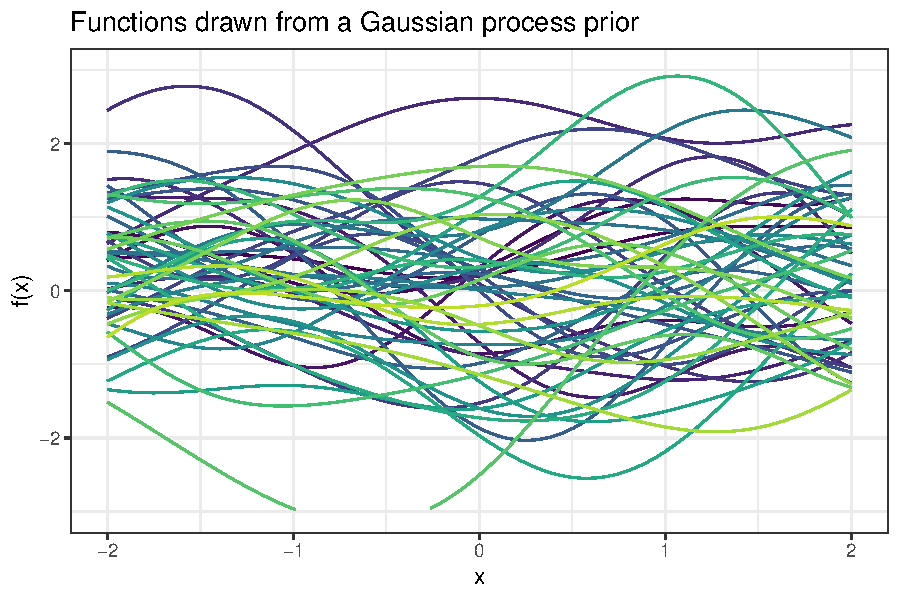
\includegraphics[width=0.5\textwidth]{figure_man/gp-sample/gp-sample-1-1.pdf}
\end{figure}

\vspace*{-0.5cm}

\begin{footnotesize}
  $^{(*)}$ We will see in a minute how distributions over functions can be specified. 
\end{footnotesize}


%%%%%%%%%%%%%%%%%%%%%%%%%%%%%%%%%%%%%%%%%%%%%%%%%%%%%%%%%%%%%%%%%%%%%%%%%%%%%%%%%%%%
\framebreak

\foreach \x in{1,2,3} {
    After observing some data points, we are allowed to sample only those functions that are consistent with the data. \\
  \begin{figure}
    \includegraphics[width=0.5\textwidth]{figure_man/gp-sample/gp-sample-2-\x.pdf}
  \end{figure}
}

%%%%%%%%%%%%%%%%%%%%%%%%%%%%%%%%%%%%%%%%%%%%%%%%%%%%%%%%%%%%%%%%%%%%%%%%%%%%%%%%%%%%
\framebreak


As we observe more and more data points, the number of functions that consistent with the data shrinks.

  \begin{figure}
    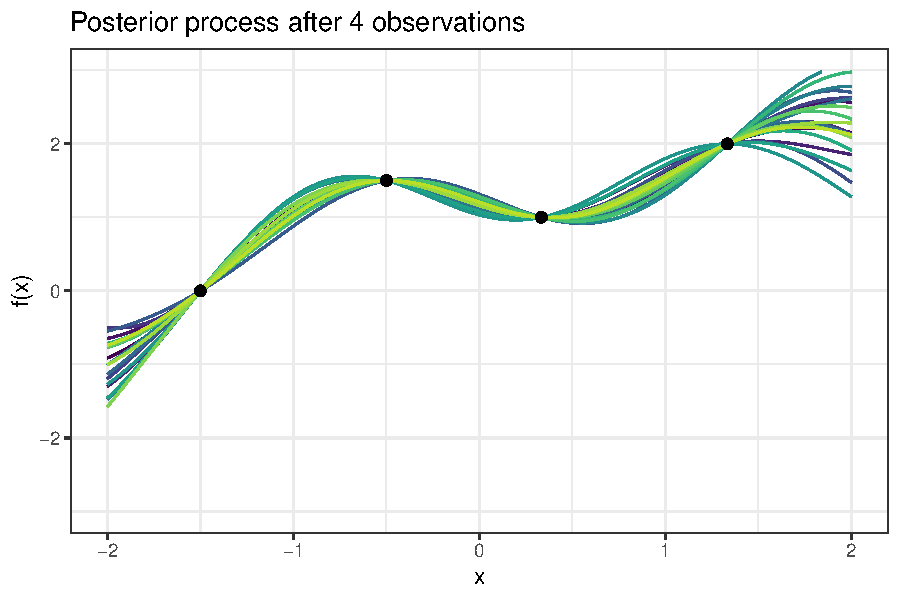
\includegraphics[width=0.5\textwidth]{figure_man/gp-sample/gp-sample-2-4.pdf}
  \end{figure}
  

%%%%%%%%%%%%%%%%%%%%%%%%%%%%%%%%%%%%%%%%%%%%%%%%%%%%%%%%%%%%%%%%%%%%%%%%%%%%%%%%%%%%
\framebreak

Intuitively, there is something like the ``mean'' and ``variance'' of a distribution over functions. 

  \begin{figure}
    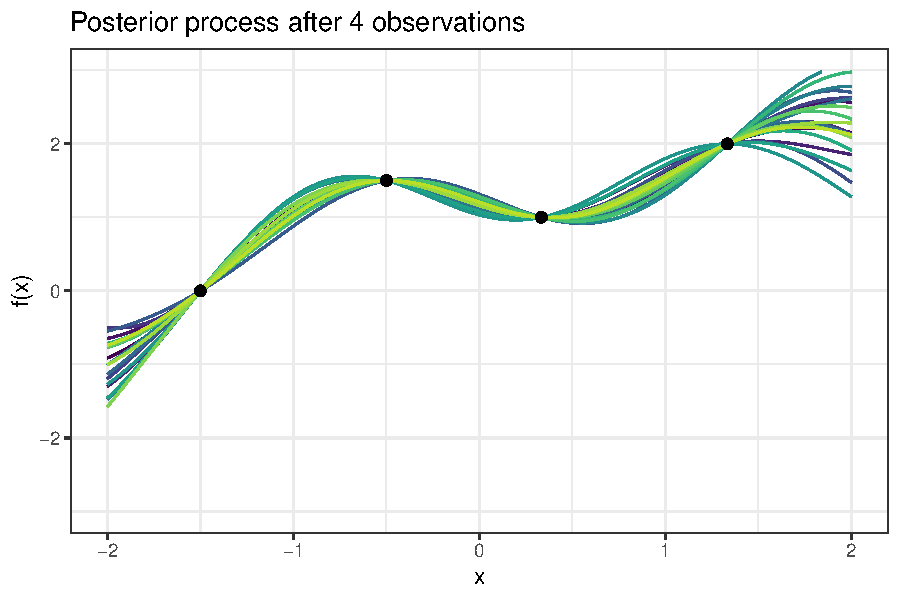
\includegraphics[width=0.5\textwidth]{figure_man/gp-sample/gp-sample-2-4.pdf}
  \end{figure}

\end{frame}
%%%%%%%%%%%%%%%%%%%%%%%%%%%%%%%%%%%%%%%%%%%%%%%%%%%%%%%%%%%%%%%%%%%%%%%%%%%%%%%%%%%%
\begin{frame}[c]{Weight-Space View vs. Function-Space View}

\begin{table}
  \begin{tabular}{cc}
  \textbf{Weight-Space View} & \textbf{Function-Space View} \vspace{4mm}\\ 
  Parameterize functions & \vspace{1mm}\\
  \footnotesize Example: $f(\x\mid\thetab) = \thetab^\top\x$ & \vspace{4mm}\\
  Define distributions on $\thetab$ & Define distributions on $f$ \vspace{4mm}\\
  Inference in parameter space $\Theta$ & Inference in function space $\Hspace$
  \end{tabular}
\end{table}  

\lz
\lz

Next, we will see how we can define distributions over functions mathematically. 


\end{frame}
%%%%%%%%%%%%%%%%%%%%%%%%%%%%%%%%%%%%%%%%%%%%%%%%%%%%%%%%%%%%%%%%%%%%%%%%%%%%%%%%%%%%

\begin{frame}[c]{}
\centering
\huge
\textbf{Distributions on Functions}
\end{frame}



\begin{frame}[c,allowframebreaks]{Discrete Functions}

For simplicity, we will firstly consider functions with finite domains. 

\lz
\lz


\begin{itemize}
\item Let $\mathcal{X} = \left\{\xI{1},\dots, \xI{n}\right\}$ be a finite set of elements and $\Hspace$ the set of all functions $h: \mathcal{X} \to\realnum$.

\lz
\lz

\item Since the domain of any $h(\cdot) \in \Hspace$ has only $n$ elements, we can represent the function $h(\cdot)$ compactly as a $n$-dimensional vector 

$$\bm{h} = \left[h\left(\xI{1}\right),\dots, h\left(\xI{n}\right)\right].$$

\end{itemize}

%%%%%%%%%%%%%%%%%%%%%%%%%%%%%%%%%%%%%%%%%%%%%%%%%%%%%%%%%%%%%%%%%%%%%%%%%%%%%%%%%%%%
\framebreak

\foreach \x in{1,2,3} {
\textbf{Example 1:} Consider function $h: \Xspace \to \Yspace$ where the input space consists of \textbf{two} points $\Xspace = \{0, 1\}$.

\vspace{.3cm}
Examples for functions that live in this space:
\vspace{.3cm}

\begin{figure}
  \includegraphics[width=0.5\linewidth]{figure_man/discrete/example_2_\x.pdf} \par
\end{figure}
}


%%%%%%%%%%%%%%%%%%%%%%%%%%%%%%%%%%%%%%%%%%%%%%%%%%%%%%%%%%%%%%%%%%%%%%%%%%%%%%%%%%%%
\framebreak

\foreach \x in{1,2,3} {
\textbf{Example 2:} Consider $h: \Xspace \to \Yspace$ where the input space consists of \textbf{five} points $\Xspace = \{0, 0.25, 0.5, 0.75, 1\}$.

\vspace{.3cm}
Examples for functions that live in this space:
\vspace{.3cm}


\begin{figure}
  \includegraphics[width=0.5\linewidth]{figure_man/discrete/example_5_\x.pdf}\par
\end{figure}
}

%%%%%%%%%%%%%%%%%%%%%%%%%%%%%%%%%%%%%%%%%%%%%%%%%%%%%%%%%%%%%%%%%%%%%%%%%%%%%%%%%%%%
%\framebreak

\foreach \x in{1,2,3} {
\textbf{Example 3:} Consider $h: \Xspace \to \Yspace$ where the input space consists of \textbf{ten} points.

\vspace{.3cm}

Examples for functions that live in this space:

\vspace{.3cm}
\begin{figure}
  \includegraphics[width=0.5\textwidth]{figure_man/discrete/example_10_\x.pdf}
\end{figure}
}

\end{frame}
%%%%%%%%%%%%%%%%%%%%%%%%%%%%%%%%%%%%%%%%%%%%%%%%%%%%%%%%%%%%%%%%%%%%%%%%%%%%%%%%%%%%
\begin{frame}[c,allowframebreaks]{Distributions on Discrete Functions}

\begin{itemize}
\item One natural way to specify a probability distribution on a discrete function $h \in \Hspace$ is to use the vector representation of the function:
$$\bm{h} = \left[h\left(\xI{1}\right), h\left(\xI{2}\right),\dots, h\left(\xI{n}\right)\right].$$ 
\lz
\item Let us consider $\bm{h}$ as a $n$-dimensional random variable. We will further assume the following normal distribution: 
$$\bm{h} \sim \normaldist\left(\bm{m}, \bm{K}\right).$$ 
\end{itemize}

\textbf{Note: }For now, we set $\bm{m} = \bm{0}$ and take the covariance matrix $\bm{K}$ as given. We will see later how they are chosen / estimated. 


%%%%%%%%%%%%%%%%%%%%%%%%%%%%%%%%%%%%%%%%%%%%%%%%%%%%%%%%%%%%%%%%%%%%%%%%%%%%%%%%%%%%
\framebreak

\foreach \x in{1,2,3} {
\textbf{Example 1 (continued):} Let $h: \Xspace \to \Yspace$ be a function that is defined on \textbf{two} points $\Xspace$. We sample functions by sampling from a two-dimensional normal variable
\vspace{-.1cm}
$$\bm{h} = [h(1), h(2)] \sim \normaldist(\bm{m}, \bm{K}).$$
\vspace{-.5cm}
\begin{figure}
  \includegraphics[width=0.3\textwidth]{figure_man/discrete/example_norm_2_\x-a.pdf} ~  \includegraphics[width=0.3\textwidth]{figure_man/discrete/example_norm_2_\x-b.pdf}
  
\begin{footnotesize}
In this example, $m = (0, 0)$ and $K = \begin{pmatrix} 1 & 0.5 \\ 0.5 & 1 \end{pmatrix}$.
\end{footnotesize}
\end{figure}
}

%%%%%%%%%%%%%%%%%%%%%%%%%%%%%%%%%%%%%%%%%%%%%%%%%%%%%%%%%%%%%%%%%%%%%%%%%%%%%%%%%%%%
\framebreak

\foreach \x in{1,2,3} {
\textbf{Example 2 (continued):} Let us consider $h: \Xspace \to \Yspace$ where the input space consists of \textbf{five} points. We sample functions by sampling from a five-dimensional normal variable
\vspace{-.1cm}
$$\bm{h} = [h(1), h(2), h(3), h(4), h(5)] \sim \normaldist(\bm{m}, \bm{K}).$$
\vspace{-.5cm}
\begin{figure}
  \includegraphics[width=0.3\textwidth]{figure_man/discrete/example_norm_5_\x-a.pdf} ~  \includegraphics[width=0.3\textwidth]{figure_man/discrete/example_norm_5_\x-b.pdf}
  \end{figure}
}


%%%%%%%%%%%%%%%%%%%%%%%%%%%%%%%%%%%%%%%%%%%%%%%%%%%%%%%%%%%%%%%%%%%%%%%%%%%%%%%%%%%%
\framebreak

\foreach \x in{1,2,3} {
\textbf{Example 3 (continued):} Let us consider $h: \Xspace \to \Yspace$ where the input space consists of \textbf{ten} points. We sample functions by sampling from a ten-dimensional normal variable
\vspace{-.1cm}
$$\bm{h} = [h(1), h(2),\dots, h(10)] \sim \normaldist(\bm{m}, \bm{K}).$$
\vspace{-.5cm}
\begin{figure}
  \includegraphics[width=0.3\textwidth]{figure_man/discrete/example_norm_10_\x-a.pdf} ~  \includegraphics[width=0.3\textwidth]{figure_man/discrete/example_norm_10_\x-b.pdf}
  \end{figure}
}

\end{frame}


%%%%%%%%%%%%%%%%%%%%%%%%%%%%%%%%%%%%%%%%%%%%%%%%%%%%%%%%%%%%%%%%%%%%%%%%%%%%%%%%%%%%
\begin{frame}[c,allowframebreaks]{The Role of Covariance Function}
\vspace{-.03cm}

The covariance controls the ``shape'' of drawn functions. Consider two extreme cases where function values are:
\vspace{-.1cm}
\begin{enumerate}
  \item[a)] strongly correlated: $\bm{K} = \begin{footnotesize}\begin{pmatrix} 1 & 0.99 & ... & 0.99 \\
  0.99 & 1 & ... & 0.99 \\
  0.99 & 0.99 & \ddots & 0.99 \\
  0.99 & ... & 0.99 & 1 \end{pmatrix}\end{footnotesize}$
  \vspace{-.4cm}
  \item[b)] uncorrelated: $\bm{K} = \id$.
\end{enumerate}

\begin{figure}
  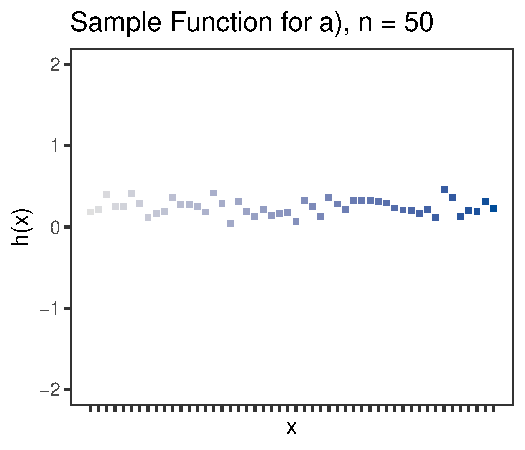
\includegraphics[width=0.31\textwidth]{figure_man/discrete/example_extreme_50-1.pdf} ~~  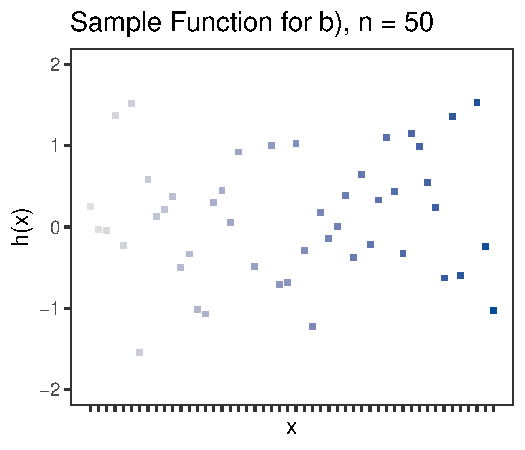
\includegraphics[width=0.31\textwidth]{figure_man/discrete/example_extreme_50-2.pdf}
\end{figure}

%%%%%%%%%%%%%%%%%%%%%%%%%%%%%%%%%%%%%%%%%%%%%%%%%%%%%%%%%%%%%%%%%%%%%%%%%%%%%%%%%%%%
\framebreak

\begin{itemize}
  \item On a numeric space $\Xspace$, ``meaningful'' functions may be characterized by the following spatial property:
\end{itemize}

\begin{displayquote}
If $\xI{i}$ and $\xI{j}$ are close in the $\Xspace$-space, their function values $f(\xI{i})$ and $f(\xI{j})$ should be close in $\Yspace$-space.
\end{displayquote}

\lz
\begin{itemize}
  \item[\faLightbulbO] In other words, if two data points are close in $\Xspace$-space, their corresponding values should be \textbf{correlated}!
  
  \lz
  
  \item[\faLightbulbO] We can enforce this condition by choosing a covariance function for which,  
\end{itemize}
 $$\bm{K}_{ij} \text{ is high, if } \xI{i} \text{ and } \xI{j} \text{ are close.}$$



%%%%%%%%%%%%%%%%%%%%%%%%%%%%%%%%%%%%%%%%%%%%%%%%%%%%%%%%%%%%%%%%%%%%%%%%%%%%%%%%%%%%
\framebreak


We can compute the entries of the covariance matrix by a function that is based on the distance between $\xI{i}$ and $\xI{j}$. For example: 

\begin{enumerate}
    \item[c)] spatial correlation: \begin{footnotesize}$K_{ij} = k(\xI{i}, \xI{j}) = \exp\left(-\frac{1}{2}\left|\xI{i} - \xI{j}\right|^2\right)$\end{footnotesize}
\end{enumerate}
  
\begin{figure}
  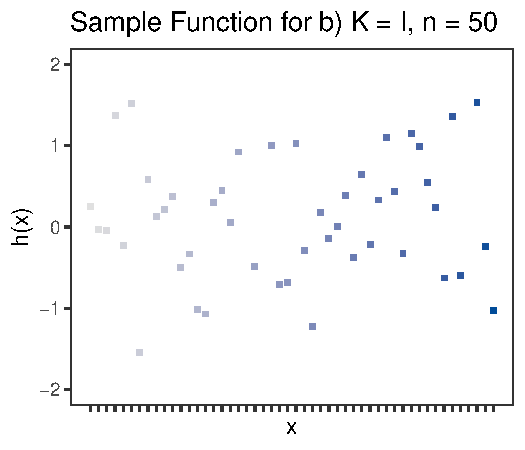
\includegraphics[width=0.3\textwidth]{figure_man/discrete/example_extreme_50-4.pdf} ~~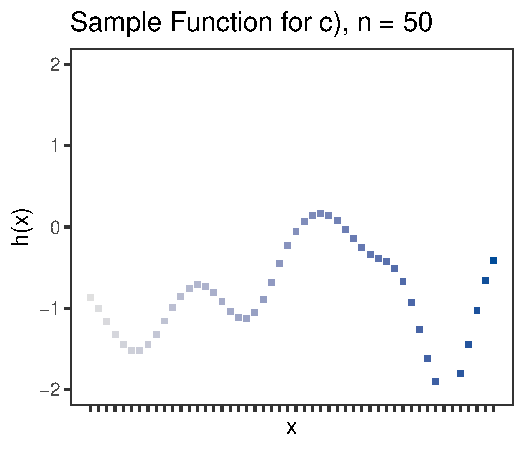
\includegraphics[width=0.3\textwidth]{figure_man/discrete/example_extreme_50-3.pdf}
\end{figure}


\begin{footnotesize}
\textbf{Note}: $k(\cdot,\cdot)$ is known as the \textbf{covariance function} or \textbf{kernel}. It will be studied in more detail later on.
\end{footnotesize}

\end{frame}

%%%%%%%%%%%%%%%%%%%%%%%%%%%%%%%%%%%%%%%%%%%%%%%%%%%%%%%%%%%%%%%%%%%%%%%%%%%%%%%%%%%%
\begin{frame}[c]{}
\centering
\huge
\textbf{Gaussian Processes}
\end{frame}

%%%%%%%%%%%%%%%%%%%%%%%%%%%%%%%%%%%%%%%%%%%%%%%%%%%%%%%%%%%%%%%%%%%%%%%%%%%%%%%%%%%%
\begin{frame}[c]{From Discrete to Continuous Functions}

\begin{itemize}
  \item We have already considered distributions on functions with discrete domain. We did so, by defining Gaussian distributions on the vector of the respective function values $$\mathbf{h} = [h(\xI{1}), h(\xI{2}),\dots, h(\xI{n})] \sim \normaldist(\bm{m}, \bm{K}).$$
  \item We can generalize this idea for $n \to \infty$.
\end{itemize}

\begin{figure}
    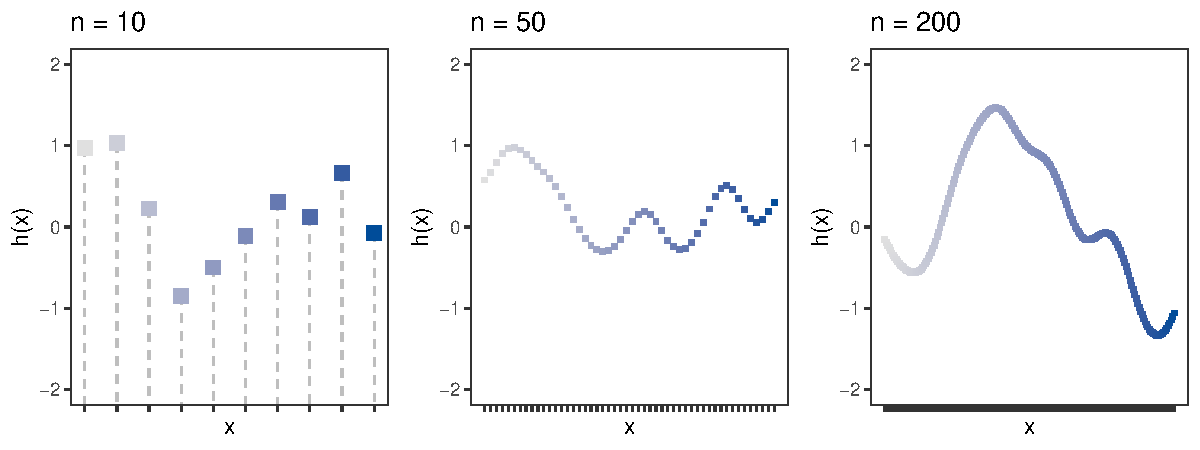
\includegraphics[width = 0.65\textwidth]{figure_man/discrete/example_limit.pdf}
  \end{figure}
\end{frame}
%%%%%%%%%%%%%%%%%%%%%%%%%%%%%%%%%%%%%%%%%%%%%%%%%%%%%%%%%%%%%%%%%%%%%%%%%%%%%%%%%%%%

\begin{frame}[c,allowframebreaks]{Gaussian Processes: Intuition}


\begin{itemize}
  \item  No matter how large $n$ is, we consider functions with discrete domains.
\vspace{.3cm}
  \item But, how can we extend our definition to functions with \textbf{continuous} domains $\Xspace \subset \realnum$?
\vspace{.3cm}
  \item Intuitively, a function $f$ drawn from a \textbf{Gaussian process} can be understood as an ``infinite'' long Gaussian random vector.
\vspace{.3cm}
  \item It is unclear how to handle an ``infinite'' long Gaussian random vector!
\end{itemize}

\vspace{.3cm}

\begin{figure}

\includegraphics[width=0.18\textwidth]{figure_man/question.png}
\end{figure}
%%%%%%%%%%%%%%%%%%%%%%%%%%%%%%%%%%%%%%%%%%%%%%%%%%%%%%%%%%%%%%%%%%%%%%%%%%%%%%%%%%%%
\framebreak

\begin{itemize}
\item Thus, it is required that for \textbf{any finite set} of inputs $\{\xI{1},\dots,\xI{n}\} \subset \Xspace$, the vector $\mathbf{f}$ has a Gaussian distribution with $\bm{m}$ and $\bm{K}$ being calculated by a mean function $m(\cdot)$ and a covariance function $k(\cdot,\cdot)$:\vspace{-.2cm}$$\bm{f} = \left[f\left(\xI{1}\right),\dots, f\left(\xI{n}\right)\right] \sim\normaldist\left(\bm{m},\bm{K}\right).$$
    
\item This property is called the \textbf{Marginalization Property}. 
\vspace{.15cm}
\begin{figure}
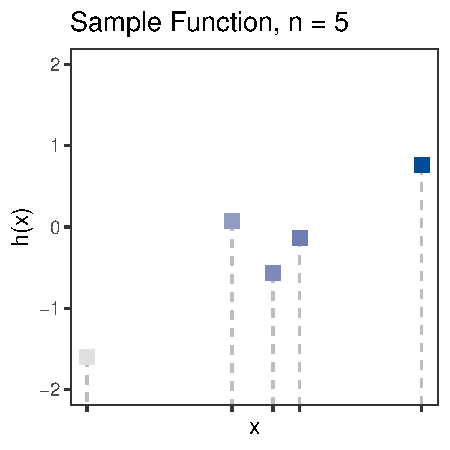
\includegraphics[width=0.2\textwidth]{figure_man/discrete/example_marginalization_5.pdf}
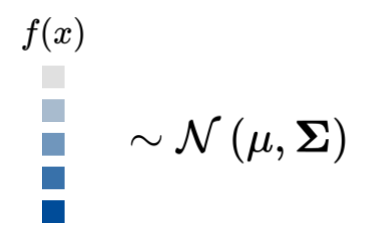
\includegraphics[width=0.3\textwidth]{figure_man/discrete/marginalization-5.png}
\end{figure}
\end{itemize}


%%%%%%%%%%%%%%%%%%%%%%%%%%%%%%%%%%%%%%%%%%%%%%%%%%%%%%%%%%%%%%%%%%%%%%%%%%%%%%%%%%%%
\framebreak

\begin{itemize}
\item Thus, it is required that for \textbf{any finite set} of inputs $\{\xI{1},\dots,\xI{n}\} \subset \Xspace$, the vector $\mathbf{f}$ has a Gaussian distribution with $\bm{m}$ and $\bm{K}$ being calculated by a mean function $m(\cdot)$ and a covariance function $k(\cdot,\cdot)$:\vspace{-.2cm}$$\bm{f} = \left[f\left(\xI{1}\right),\dots, f\left(\xI{n}\right)\right] \sim\normaldist\left(\bm{m},\bm{K}\right).$$
    
\item This property is called the \textbf{Marginalization Property}. 
\vspace{.15cm}
\begin{figure}
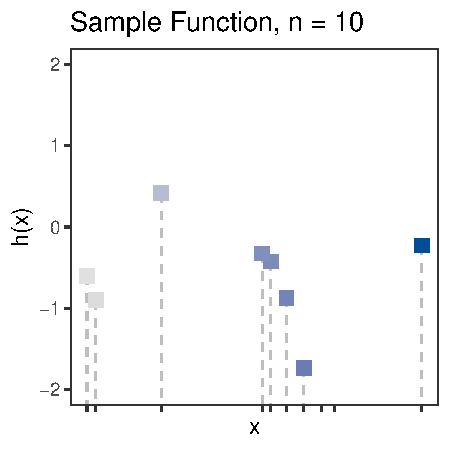
\includegraphics[width=0.2\textwidth]{figure_man/discrete/example_marginalization_10.pdf}
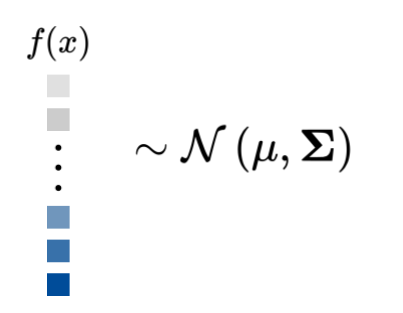
\includegraphics[width=0.3\textwidth]{figure_man/discrete/marginalization-more.png}
\end{figure}
\end{itemize}


%%%%%%%%%%%%%%%%%%%%%%%%%%%%%%%%%%%%%%%%%%%%%%%%%%%%%%%%%%%%%%%%%%%%%%%%%%%%%%%%%%%%
\framebreak


\begin{itemize}
\item Thus, it is required that for \textbf{any finite set} of inputs $\{\xI{1},\dots,\xI{n}\} \subset \Xspace$, the vector $\mathbf{f}$ has a Gaussian distribution with $\bm{m}$ and $\bm{K}$ being calculated by a mean function $m(\cdot)$ and a covariance function $k(\cdot,\cdot)$:\vspace{-.2cm}$$\bm{f} = \left[f\left(\xI{1}\right),\dots, f\left(\xI{n}\right)\right] \sim\normaldist\left(\bm{m},\bm{K}\right).$$
    
\item This property is called the \textbf{Marginalization Property}. 
\vspace{.15cm}
\begin{figure}
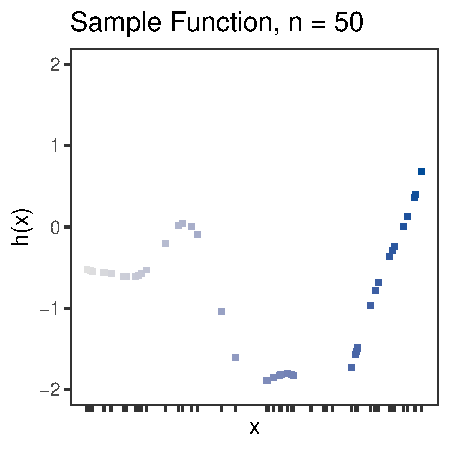
\includegraphics[width=0.2\textwidth]{figure_man/discrete/example_marginalization_50.pdf}
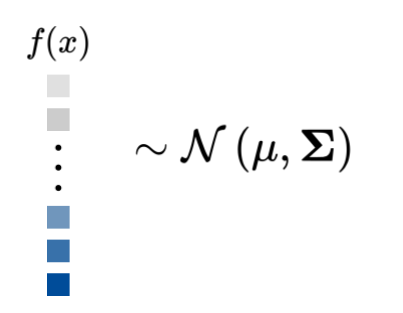
\includegraphics[width=0.3\textwidth]{figure_man/discrete/marginalization-more.png}
\end{figure}
\end{itemize}
\end{frame}

%%%%%%%%%%%%%%%%%%%%%%%%%%%%%%%%%%%%%%%%%%%%%%%%%%%%%%%%%%%%%%%%%%%%%%%%%%%%%%%%%%%%
\begin{frame}[c,allowframebreaks]{Gaussian Processes: Formal Definitions}

\begin{itemize}
\item The above intuitive explanation is formally defined as follows. 
\end{itemize}

\vspace{.7cm}

\begin{displayquote}
A function $f(\x)$ is generated by a Gaussian process $\gp$ if for \textbf{any finite} set of inputs $\left\{\xI{1},\dots,\xI{n}\right\}$, the associated vector of function values has a Gaussian distribution:
$$\bm{f} = \left(f(\xI{1}),\dots, f(\xI{n})\right) \sim\normaldist\biggl(\textbf{m},\textbf{K}\biggr),$$ with 

$$\textbf{m}:= \left(m\left(\xI{i}\right)\right)_{i}, \quad
\textbf{K}:= \left(k\left(\xI{i}, \xI{j}\right)\right)_{i,j},$$ 

where $m(\x)$ is called mean function and $k(\x, \x^\prime)$ is called covariance function.
\end{displayquote}

%%%%%%%%%%%%%%%%%%%%%%%%%%%%%%%%%%%%%%%%%%%%%%%%%%%%%%%%%%%%%%%%%%%%%%%%%%%%%%%%%%%%
\framebreak


\begin{itemize}

\item A GP is \textbf{completely specified} by its mean and covariance functions.
\vspace{.2cm}

\item The mean function $m(\x)$ and the covariance function $k(\x, \x^\prime)$ of a real process $f(\x)$ are defined as:
\vspace{-.4cm}
\begin{eqnarray*}
m(\x) &=& \expectation[f(\x)] \\
k(\x, \x^\prime) &=& \expectation\biggl[\left( f(\x) - \expectation[f(\x)] \right) \left( f(\x^\prime) - \expectation[f(\x^\prime)] \right)\biggr]
\end{eqnarray*}

\vspace{.2cm}

\item We denote a GP by
\vspace{-.1cm}
$$f(\x) \sim \gp\left(m(\x), k\left(\x, \x^\prime\right)\right) $$
\end{itemize}

\vspace{.3cm}

\textbf{Note:} For now, we assume $m(\x)\equiv 0$. This is not a drastic limitation. In fact, it is common to consider GPs with a zero mean function.

\end{frame}
%%%%%%%%%%%%%%%%%%%%%%%%%%%%%%%%%%%%%%%%%%%%%%%%%%%%%%%%%%%%%%%%%%%%%%%%%%%%%%%%%%%%
\begin{frame}[c,allowframebreaks]{Sampling from a Gaussian Process Prior}

\begin{itemize}

\item We can draw functions from a Gaussian process prior. To do so, consider $f(\x) \sim \gp\left(0, k(\x, \x^\prime)\right)$ with the squared exponential covariance function $^{(*)}$

$$
k(\x, \x^\prime) = \exp\left(-\frac{1}{2\ls^2}\|\x - \x^\prime\|^2\right), ~~ \ls = 1.
$$

\lz

\item This covariance function specifies the Gaussian process completely. 

\end{itemize}

\vspace{2cm}
\begin{footnotesize}
$^{(*)}$ We will talk later about different choices of covariance functions. 
\end{footnotesize}


%%%%%%%%%%%%%%%%%%%%%%%%%%%%%%%%%%%%%%%%%%%%%%%%%%%%%%%%%%%%%%%%%%%%%%%%%%%%%%%%%%%%
\framebreak

To visualize a sample function, we 
\begin{itemize}
  \item choose a large number of equidistant points: $\left\{\xI{1},\dots,\xI{n}\right\}$,
  \item compute their corresponding covariance matrix by plugging in all pairs of $\xI{i}$ and $\xI{j}$ in $\textbf{K} = \left(k\left(\xI{i}, \xI{j}\right)\right)_{i,j}$,
  \item sample from a Gaussian $\bm{f} \sim \normaldist (\bm{0}, \bm{K})$.
\end{itemize}

\begin{figure}
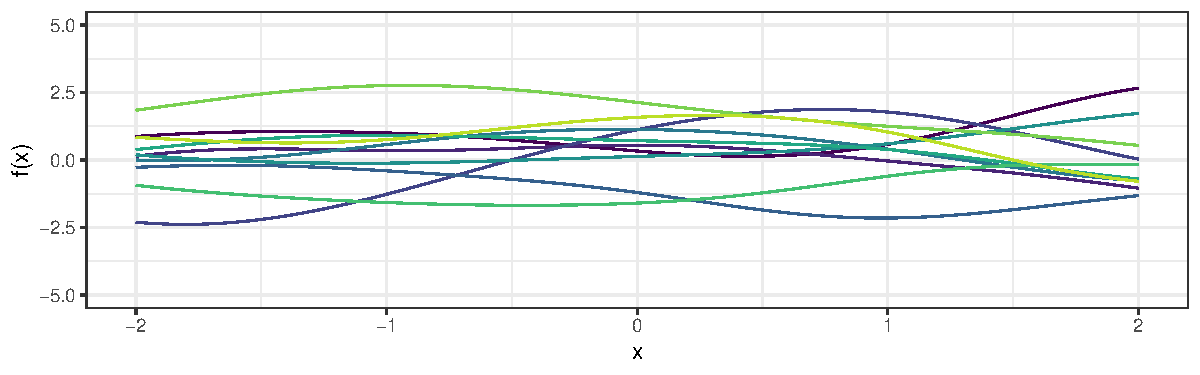
\includegraphics[width=0.6\textwidth]{figure_man/gp-sqexp-1-1.pdf}
\begin{footnotesize}
\caption*{We draw $10$ times from the Gaussian, to get $10$ different samples. Since we specified the mean function to be zero, the drawn functions have a zero mean.}
\end{footnotesize}
\end{figure}

\end{frame}

%%%%%%%%%%%%%%%%%%%%%%%%%%%%%%%%%%%%%%%%%%%%%%%%%%%%%%%%%%%%%%%%%%%%%%%%%%%%%%%%%%%%
\framebreak

\begin{frame}[c]{}
\centering
\huge
\textbf{Gaussian Processes as an Indexed Family}
\end{frame}


%%%%%%%%%%%%%%%%%%%%%%%%%%%%%%%%%%%%%%%%%%%%%%%%%%%%%%%%%%%%%%%%%%%%%%%%%%%%%%%%%%%%
\begin{frame}[c]{Gaussian Processes as an Indexed Family}

\begin{itemize}
\item A Gaussian process is a special case of a \textbf{stochastic process} which is defined as a collection of random variables indexed by some index set (also called an \textbf{indexed family}).
\lz
\item What does it mean?
\lz
\item An \textbf{indexed family} is a mathematical function (or ``rule'') that maps indices $t \in T$ to objects in $\mathcal{S}$.
\end{itemize}
\lz


\begin{displayquote} 
\textbf{Definition:} an \textbf{index family} (or a family of elements in $\mathcal{S}$ indexed by $T$) is a surjective function that is defined as follows:
\vspace{-.2cm}
\begin{eqnarray*}
s: T &\to& \mathcal{S} \\
   t &\mapsto& s_t = s(t) 
\end{eqnarray*}

\end{displayquote}

\end{frame}


%%%%%%%%%%%%%%%%%%%%%%%%%%%%%%%%%%%%%%%%%%%%%%%%%%%%%%%%%%%%%%%%%%%%%%%%%%%%%%%%%%%%
\begin{frame}[c,allowframebreaks]{Index Family}

Some simple examples for indexed families are:
\begin{columns}[T]
\begin{column}{.5\textwidth}
\vspace*{1cm}
  \begin{itemize}
  \item Finite sequences (lists): $T = \{1, 2,\dots, n\}$ and $\left(s_t\right)_{t \in T}\in\realnum $
  \vspace{2.5cm}
  \item Infinite sequences: $T = \natnum$ and $\left(s_t\right)_{t \in T} \in \realnum$
  \end{itemize}
  
\end{column}
\begin{column}{.35\textwidth}
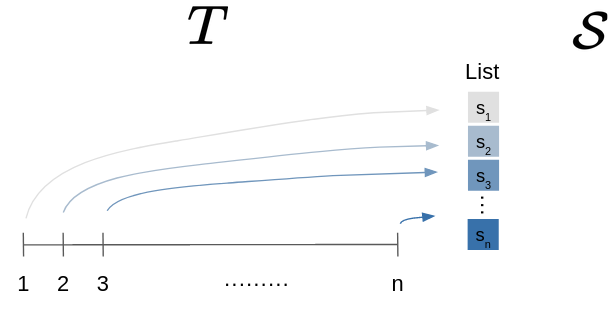
\includegraphics[width=\textwidth]{figure_man/indexed_family/indexed_family_1.png}\\
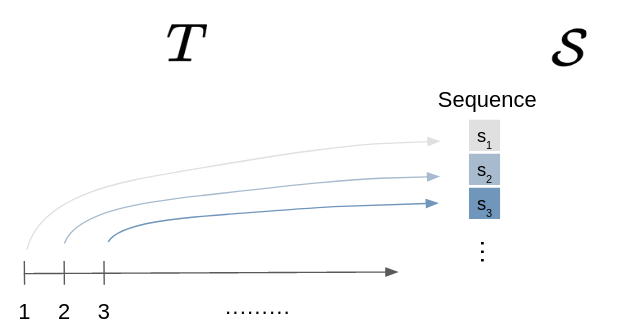
\includegraphics[width=\textwidth]{figure_man/indexed_family/indexed_family_2.png}
\end{column}
\end{columns}

%%%%%%%%%%%%%%%%%%%%%%%%%%%%%%%%%%%%%%%%%%%%%%%%%%%%%%%%%%%%%%%%%%%%%%%%%%%%%%%%%%%%

%%%%%%%%%%%%%%%%%%%%%%%%%%%%%%%%%%%%%%%%%%%%%%%%%%%%%%%%%%%%%%%%%%%%%%%%%%%%%%%%%%%%
\framebreak


But the indexed set $\mathcal{S}$ can be something more complicated, for example functions or \textbf{random variables} (RV):

\begin{columns}[T]
\begin{column}{.5\textwidth}
\vspace*{1cm}
  \begin{itemize}
    \item $T = \{1,\dots, m\}$, $Y_t$'s are RVs: Indexed family is a random vector.
    \vspace*{0.4cm}
    \item $T = \{1,\dots, m\}$, $Y_t$'s are RVs: Indexed family is a stochastic process in discrete time. 
    \vspace*{0.4cm}
    \item $T = \intnum^2$, $Y_t$'s are RVs: Indexed family is a 2D-random walk.
  \end{itemize}
  
\end{column}
\begin{column}{.35\textwidth}
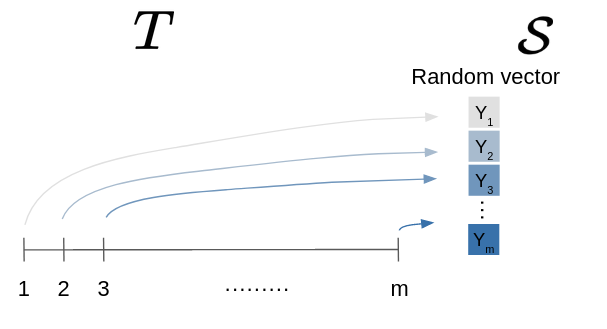
\includegraphics[width=\textwidth]{figure_man/indexed_family/indexed_family_4.png}\\
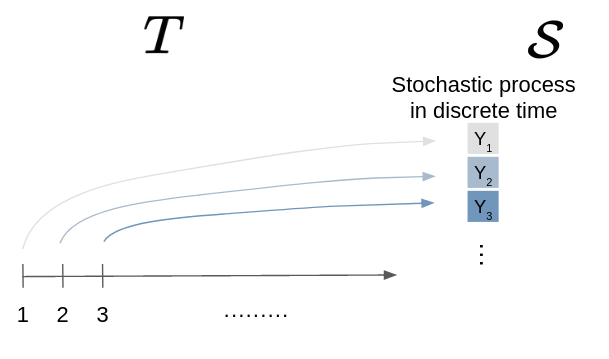
\includegraphics[width=\textwidth]{figure_man/indexed_family/indexed_family_3.png}
\end{column}
\end{columns}



\begin{itemize}
  \item A Gaussian process is also an indexed family, where the random variables $f(\x)$ are indexed by the input values $\x\in\Xspace$. 
  \item Importantly, any indexed (finite) random vector has a multivariate Gaussian distribution (which comes with all the nice properties of Gaussianity!). 
\end{itemize}

\lz

\begin{figure}
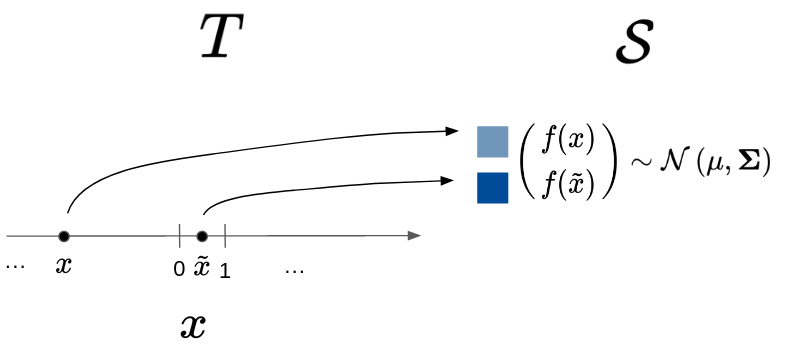
\includegraphics[width=0.5\textwidth]{figure_man/indexed_family/indexed_family_5.png}\par
\begin{footnotesize}
Visualization for a one-dimensional $\Xspace$.
\end{footnotesize}
\end{figure}


%%%%%%%%%%%%%%%%%%%%%%%%%%%%%%%%%%%%%%%%%%%%%%%%%%%%%%%%%%%%%%%%%%%%%%%%%%%%%%%%%%%%
\framebreak

\begin{itemize}
  \item A Gaussian process is also an indexed family, where the random variables $f(\x)$ are indexed by the input values $\x\in\Xspace$. 
  \item Importantly, any indexed (finite) random vector has a multivariate Gaussian distribution (which comes with all the nice properties of Gaussianity!). 
\end{itemize}

\lz

\begin{figure}
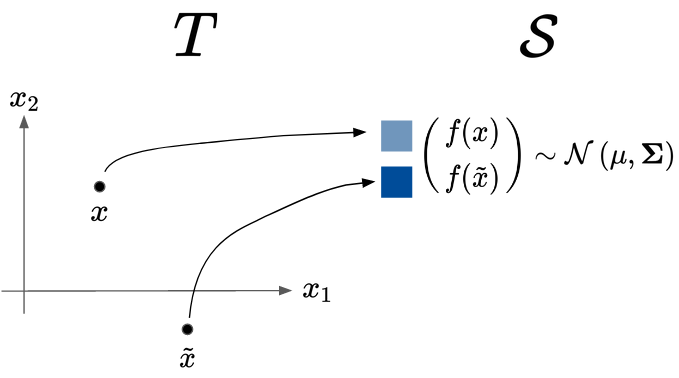
\includegraphics[width=0.4\textwidth]{figure_man/indexed_family/indexed_family_6.png}\par
\begin{footnotesize}
Visualization for a two-dimensional $\Xspace$.
\end{footnotesize}
\end{figure}

%%%%%%%%%%%%%%%%%%%%%%%%%%%%%%%%%%%%%%%%%%%%%%%%%%%%%%%%%%%%%%%%%%%%%%%%%%%%%%%%%%%%
\framebreak

%%%%%%%%%%%%%%%%%%%%%%%%%%%%%%%%%%%%%%%%%%%%%%%%%%%%%%%%%%%%%%%%%%%%%%%%%%%%%%%%%%%%
\framebreak

%%%%%%%%%%%%%%%%%%%%%%%%%%%%%%%%%%%%%%%%%%%%%%%%%%%%%%%%%%%%%%%%%%%%%%%%%%%%%%%%%%%%
\framebreak


%%%%%%%%%%%%%%%%%%%%%%%%%%%%%%%%%%%%%%%%%%%%%%%%%%%%%%%%%%%%%%%%%%%%%%%%%%%%%%%%%%%%
\framebreak



\end{frame}


\end{document}
